\chapter[Diva code]{Diva code}
%-----------------------------
\hypertarget{DIVACODE}{}

The engine of \diva is a set of Fortran subroutines driven by local input and output files (\file{fort.*}).
This chapter is dedicated to the description of these programs, in order to allow the advanced user to adapt the code according to his needs.

\minitoc


\section[Fortran code]{Fortran code \expert}
%---------------------

The Fortran programs are sorted according to their purpose: 

\begin{lstlisting}[style=Bash]
[charles@gher13 Fortran] tree -d -L 1
.
|-- Calc
|-- Extensions
|-- Mesh
|-- NC
|-- NoPlplot
|-- Pipetest
|-- Plplot
|-- Stabil
`-- Util

9 directories
\end{lstlisting}

\subsection[Calculation programs]{Calculation programs [\directory{src/Fortran/Calc}]}
%------------------------------------------------------------------------------------------

The main file of the Fortran code is \file{diva.f}: this routine calls the subroutines enumerated below, in order to perform a \diva analysis:
\vspace{.15cm}
\begin{description}
\item[\file{mathpr.f}]: describes the mathematical problem.
\item[\file{topolo.f}]: describes the topology of the finite element grid.
\item[\file{meshgn.f}]: generates a square finite element mesh on a regular grid.
\item[\file{datapr.f}]: input of data to be fitted by spline smoothing.
\item[\file{bcondi.f}]: Dirichlet boundary conditions to be fixed.
\item[\file{constr.f}]: input of information for constraint implementation.
\item[\file{solver.f}]: builds and solves the global linear finite element system.
\item[\file{stores.f}]: storage of the solution.
\item[\file{esterr.f}]: estimates the analysis error (same grid as the analysis).
\item[\file{coord.f}]: coordinate change (longitude, latitude) to $(x,y)$ and $(x,y)$ to (longitude, latitude) if requested.
\item[\file{gcvfac.f}]: estimates the analysis error by generalized cross-validation.  
\item[\file{dataqc.f}]: data quality check: estimates of expected data-analysis differences.   
\item[\file{covar.f}]: calculation of \diva kernel for subsequent error fields.        
\end{description}
\vspace{.15cm}
Other routines related to \diva calculation:
\begin{description}
\item[\file{allody.f}]: dynamical allocation of storage area in $S$ or $L$ vector.
\item[\file{bilinin.f}]: interpolates from a regular field into $xt,yt$; called in \file{constr.f}.
\item[\file{finca.f}]: finds in which region is one point.
\item[\file{optimi.f}]: subroutines used for the optimisation:

\begin{itemize}

\item[] \file{divesp.f}: subdivides the space for optimisation;
\item[] \file{sizes2.f}: computes the size of the space for elements of type 2;
\item[] \file{sizes3.f}: computes the size of the space for elements of type 3;
\item[] \file{repel2.f}: distributes the elements of type 2 in kntc table;
\item[] \file{repel3.f}: distributes the elements of type 2 in kntc table;
%\item \file{findca.f}: finds in which region is one point;
\item[] \file{locpt2opti.f}:  locates the $(x,y)$ point in the structure (for ityp=2);
\item[] \file{locpt3opti.f}:  locates the $(x,y)$ point in the structure (for ityp=3);
\item[] \file{sortdopti.f}:  sorts the data according to the sequence of elements;
\item[] \file{qs2i1r.f}:  quick Sort algorithm for \file{sortdopti} (from \url{www.netlib.org});
\item[] \file{calpsoopti}: computes pseudo data sets for error estimates;
\item[] \file{fcorropti.f}:  part of \file{calpsoopti};
\item[] \file{tabess.f}: tabulates the Bessel function for the calculation of error.
\end{itemize}


\item[\file{repeltest.f}]: called in \file{datapr.f}
\item[\file{shapef.f}]: evaluation of the shape functions at Gauss points.
\item[\file{utilit.f}]: utility routines.
\item[\file{uur.f}]: for the advection constraint.
\item[\file{uwrit2.f}]: writes the field $C(I,J,K)$.  
\item[\file{varl.f}]: for variable correlation length.
\item[\file{vtools.f}]: various subroutines: 
\begin{itemize}
\item[]  \file{intsec}: calculate center coordinates of quadrangular element;
\item[]  \file{istria}: check if one point lies inside a triangle;
\item[]  \file{prskyh}: print a vector to check.
\end{itemize}

\end{description}


\subsection[Mesh programs]{Mesh programs [\directory{src/Fortran/Mesh}]}
%--------------------------------------------------------------------

Files related to the generation of coastlines:
\begin{description}
\item[\file{contourcheck.f}]: check the format of an existing contour file (no repeated points, no crossing, contour not too fine).
\item[\file{contourgen.f}]: create contours based on topography;
\item[\file{coa2cont.f}]: go from ODV \file{.coa} files (see documentation of ODV) to \diva \file{coast.cont} files, using a resolution comparable to the specified gridded output of \command{divacalc}.
\end{description}

Files related to mesh generation:
\begin{description}
\item[\file{generopt.f}]: generate a multi-connex 2D mesh with the \textit{Delaunay tri\-angu\-la\-tion};
\item[\file{generopt4.f}]: same as generopt but in real*4 precision;
\item[\file{generopt8.f}]: same as generopt but in real*8 precision.
\end{description}


\subsection[Pipetest]{Pipetest [\directory{src/Fortran/Pipetest}]}
% -----------------------------------------------------------

File \file{piperw.f} checks if \textit{pipes} are supported by your \diva installation. Pipes support is automatically tested when you run \command{divatest} (Section~\ref{sec:divatest}). Issues with pipes were observed with some versions of the gfortran compiler.

\subsection[Utilities]{Utilities [\directory{src/Fortran/Util}]}
% -----------------------------------------------------------

\begin{description}
\item[\file{alpha.f}] computes the values of $\alpha_{0}$ and $\alpha_1$.

\item[\file{calcest.f}]: from relative weight on data points (data file \file{fort.44}) and generalized cross validator value (available in \file{./output/gcvval.dat}), produces the file containing the expected misfit value at data locations (\file{fort.76}), to be used by \texttt{look\-for\-outliers.a} for outliers detection. Used in \command{divaqcter}.

\item[\file{calcestbis.f}]: from relative weight on data points (data file \file{fort.44}) and the trace 
of the analysis matrix (available in \file{./\-output/\-gcvval.dat}) produces the file
containing the expected misfit value at data locations (\file{fort.76}), to be 
used by \texttt{look\-for\-outliers.a} for outliers detection. Used in \command{divaqcbis}.

\item[\file{calcmu.f}] computes the coefficient $\mu$ knowing  the characteristic length $L$ and the signal-to-noise ratio $\snr$.

\item[\file{cverror.f}]: rms error by cross validation (called in \command{divacvrand}).

\item[\file{cverroraii.f}]: same as \file{cverror.f} but using the \textit{missing-data lemma} (called in \command{divacv}).

\item[\file{cvtotalerror.f}]: sum of the different error contributions, in the resampling case (called in \command{divacvrand}).


\item[\file{datacheck.f}]: take the input data \file{./input/data.dat} and eliminates 
all data that fall outside the bounding box of the contours (called in \command{divadataclean}). 

\item[\file{datadiff.f}]: compute data anomaly (called in \command{divaanom})


\item[\file{dbdb2diva.f}]: converts topography extracted from Navy website into \diva compatible format (Section~\ref{sec:toponavy}).

\item[\file{gebco2diva.f}]: converts topography extracted from GEBCO website into \diva compatible format (Section~\ref{sec:topogebco}).


\item[\file{findmin.f}]: from a list of values (SNR, GCV, data-variance) found in \file{fort.11}, tries 
to find by local parabolic interpolation the minimum of GCV and the place SNR where it is found.

Points do not need to be ordered. Output (\file{fort.12}) contains the 
expected value of $\snr$ in which GCV is minimal as well as the \texttt{VARBAK} 
value. Used in \command{divagcv}.

Called in \command{divacv},\command{divacvrand} and\command{divagcv}.


\item[\file{fitlsn.f}]: from the data file (\file{fort.10}) and information on coordinate change and 
reference field (\file{fort.11}), tries to fit the \textit{Bessel covariance function} to the data covariance (called in \command{divafit}).

Outputs:\\
\file{fort.66} contains the correlation length and an rough estimate of the signal-to-noise ratio;\\
\file{fort.99} contains the data-covariance over all distances;\\ 
\file{fort.98} contains the data covariance as a function of data-distance as well as the corresponding fit over distances up to the correlation length.

\item[\file{forgnuplot*.f}] consists in nine files for preparing the outputs to be viewed with the help of \gnuplot (see Section~\ref{sec:visugnuplot}). 

\item[\file{griddef.f}] creates the file \file{GridInfo.dat}, of which the content is used for writing the NetCDF output.

\item[\file{lceleme.f}] computes the mesh characteristic length (called in \command{divacck} and \command{divamesh}).

\item[\file{lookforoutliers.f}] checks if there is outliers in the data provided for the analysis (called in \command{divacalc}, \command{divaqcbis} and \command{divaqcter}).

\item[\file{multiply.f}] does what its name says (called in \command{divarefe}).

\item[\file{subsampling.f}] creates a subsampling of the data (called in \command{dvsample}).

\item[\file{sumgrid.f}] performs the sum of two gridded fields in GHER format (called in \command{divasumup}).

\item[\file{sumup.f}] performs the sum element by element of two ascii files (called in \command{divasumup}).

\item[\file{topoprep.f}] makes easier the generation of the topography using a collection of local measurements (called in \command{divatopo}).

%\end{listept}
\end{description}

\paragraph{Remark:} grid definition for users is based on an origin which is the first grid point. 
In the code, \texttt{xori} and \texttt{yori} are defined by $x_i=$ \texttt{xori} $+i \Delta x$ (and is thus shifted one grid space to the left compared to the user origin). Input file \file{fort.13} is modified from the \file{param.par} grid information by \texttt{griddef.a} accordingly, while \file{GridInfo.dat} contains the user grid as defined in \file{param.par}.

% -----------------------------------------------------------------------------------

\subsection[NetCDF output]{NetCDF output [\directory{src/Fortran/NC}]}


\index{NetCDF}
Three files allow getting an output in NetCDF format:\\ 
\file{netcdfoutputfield.f}, \file{netcdfoutputerror.f}, \file{netcdfoutput.f}. 

The two first routines write the analysed and the error fields in two different NetCDF files: \file{anlysed\_field.nc} and \file{error\_field.nc}. The last programs generates \file{results.nc} which contains both the analysis and the error fields. The information required for the coordinates (xorigin, y origin, dx, dy, xend, yend) are read from \file{GridInfo.dat}.

\begin{exfile}[H]
1\\
1\\
.5\\
 .5\\
100\\
100
\caption{\file{GridInfo.dat}}
\end{exfile}


\subsection[GUI programs]{GUI programs [\directory{src/Fortran/Extensions}]}
%-------------------------------------------------------------------------

The graphical interface requires some particular routines:
\begin{description}
\item[\file{extract.f}]: interface to select or extract Data from MODB and MED formatted databases.
\vspace{.25cm}
\item[\file{fem3d.f}] is based upon a mesh file and a bathymetry file (regular grid in GHER format); it creates a result file containing information to determinate if a mesh is in land or is sea, for a given depth.
\vspace{.25cm}
% -----------------------------------------------------------------------------------
\item[\file{concat.f}] is used to create the 3D file from the 2D files.
\item[\file{stiff.f}] generates the rigidity file (\file{fort.60}) in the 3D case.
\item[\file{mask.f}] masked the solution according to the bathymetry and the depth.
\item[\file{sum.f}] writes the sum of two fields (with same dimensions) in GHER format.
\item[\file{substref.f}] subtracts the reference field to the computed solution (only available when using the \textit{semi-normed} reference field).
\vspace{.25cm}
\item[\file{header2.f}] and \file{visu.f} are subroutines to visualize the data, the mesh and the solution (requires the \plplot\, library). Two versions of \file{visu.f} are provided: one is located in \directory{diva-\divaversion/\-src/\-Fortran/\-PlPlot} and the other in \directory{src/\-Fortran/\-NoPlPlot}. The first can be compiled only if you have installed the \plplot library on your computer (for now, only under Linux).
\end{description}



% --------------------------------------------------------------------------------------------
\section{Input and output files for the executables}
%-------------------------------

This section describes the input and output files \file{fort.*} related to the executables or binaries, which are the files ending by \texttt{.a} and located in \directory{GODIVA\_mm\_yyyy/DIVA3D/bin/}. 


\subsection{Mesh generation: \texttt{generopt.a}}		
%------------------------------------------------


\subsubsection{Files readed as input}			
  
\begin{description}
\item[\file{fort.10}:] coast file (identical to \file{coast.cont}), see example file with description, case of a square island in a square sea.	\item[\file{fort.11}:]	the parameters required for the mesh generation.		
\end{description}
				
\subsubsection{Files produced as output}

\begin{description}

\item[\file{fort.22}:] contains the finite-element\index{Finite-elements} mesh, as described here:
%---------------------------------------------------
\begin{enumerate}
\item the first part of the file has three columns: the first column gives the numbers of the nodes; the second and third ones give the $x-$ and $y-$coordinates of the nodes, respectively. \\
\example first line indicates that node no.~1 is located in $(-1,-1)$.
\item the second part is composed of only one column, which indicates the numbers of the interfaces;
\item the last part has six columns: columns 1, 3 and 5 specify the line numbers where the coordinates of the triangle points can be found; columns 2, 4 and 6 specify the interfaces numbers of the considered element.\\
\example the last line says that the last elements has its coordinates in lines 2, 3 and 5, \textit{i.e.}, at has points $(1,-1)$, $(1,1)$ and $(-0.333333343  0.333333343)$; it also says that this element is composed of interfaces no.~13, 8 and 12.
\end{enumerate}
%---------------------------------------------------


%\begin{minipage}{.4\textwidth}{

\begin{exfile}[htpb]
\begin{footnotesize}
\texttt{1 -1. -1.\\
 9  1. -1.\\
 4  1.  1.\\
 10 -1.  1.\\
 7 -0.333333343  0.333333343\\
 5\\
 11\\
 6\\
 12\\
 8\\
 2\\
 13\\
 3\\
 3 -6 4 -7 5 -8\\
 4 -9 1 -10 5 -7\\
 1 -11 2 -12 5 -10\\
 2 -13 3 -8 5 -12
} 
\end{footnotesize}
\caption{fort.22\label{fig:fort22}}
\end{exfile}

%\end{minipage}
%\begin{minipage}{.6\textwidth}

\begin{figure}[H]
\centering
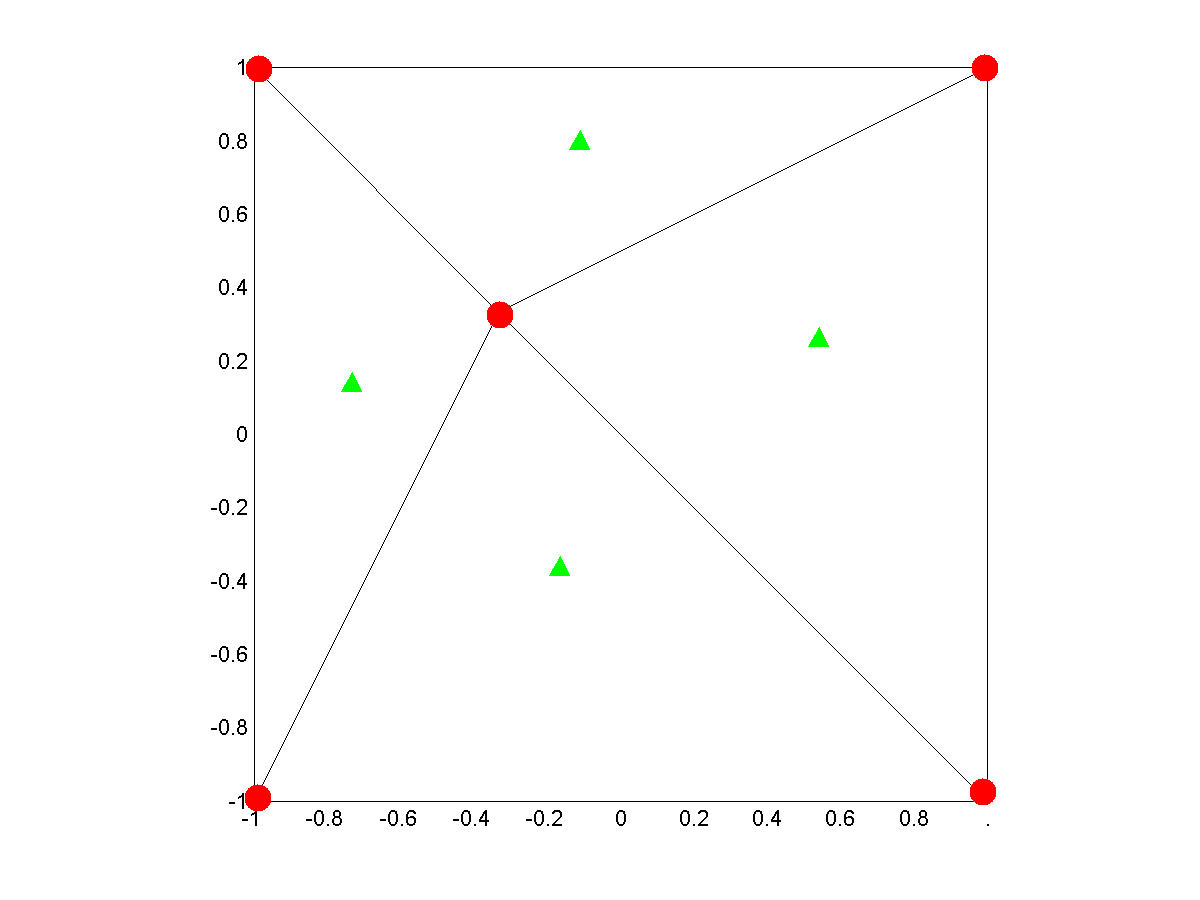
\includegraphics[width=.7\textwidth]{SimpleMesh_mesh}
\caption[Example of simple mesh]{Example of simple mesh corresponding to file \file{fort.22}.}
\end{figure}


\item[\file{fort.23}:] contains the topological parameters: 
\begin{enumerate}
\item total number of vertex nodes (red dots);
\item total number of interfaces (black lines);  
\item total number of elements (green triangles).
\end{enumerate}

\begin{exfile}[H]
\begin{verbatim}
 5
 8
 4
 \end{verbatim}
\caption{fort.23\label{fig:fort23}}
\end{exfile}
 
\end{description}

%--------------------------------------------------------------------
\subsection{\diva interpolation: \texttt{diva.a}}

\subsubsection{Files read as input}
				
\begin{description}
\item[\file{fort.10}:]			\directory{divawork} organizer, defining which modules to use and how, including several parameters.	
\item[\file{fort.11}:]			finite-element mesh, copy of the \file{fort.22} produced by \texttt{generopt.a}.					
\item[\file{fort.12}:]			$\alpha_0$ and $\alpha_1$, calculated as: 
	 	\[\alpha_0=\frac{1}{L^{4}}\quad \textrm{and}  \quad  \alpha_1 =\frac{2}{L^{2}}.	\]				
\item[\file{fort.13}:]			characteristics of the regular output grid.					
\item[\file{fort.20}:]			data file; 4 columns: $|X|Y|data(X,Y)|\mu|$, where  
		\[ \mu = 4\,\pi\,\frac{\snr}{L^{2}},\]
	  with $\snr$, the signal-to-noise ratio.				
\item[\file{fort.79}:]			coordinates where analysed field values are requested; 2 columns separated by space: $|X|Y|$. 					
\item[\file{fort.15}:]			parameter \texttt{varbak}, variance of the background field, set as $=0$ will avoid calculating error field.						
\end{description}								
	 
\begin{exfile}[H]
coord 1\\
0\\
mathpr 1\\
2  -> ITYP\\
0  -> ISYM\\
2  -> IPB\\
topolo 1\\
 158 -> Number of Vertex Nodes\\
 426 -> Number of Interface Nodes\\
 268 -> Number of Elements\\
datapr 1\\
1\\
solver 1\\
0\\
stores 1\\
1  -> 1 if normal or semi-normed final, otherwise 3\\
esterr 1\\
stopex\\
\caption{fort.10}
\end{exfile}
	  
	  
\begin{exfile}[H]
0.0001  -> alpha0\\
0.02  -> alpha1
\caption{fort.12}
\end{exfile}

\begin{exfile}[H]
0  0  -> xorigin, yorigin\\
1  1  -> dx, dy\\
100  100  -> nx, ny\\
-99999  -> Exclusion Value
\caption{fort.13}
\end{exfile}

\begin{exfile}[H]
\tt
90 90 1 12.5663706\\
90 80 1 12.5663706\\
90 70 1 12.5663706\\
$$\cdots$$\\
16 30 2 12.5663706\\
16 20 2 12.5663706\\
16 10 2 12.5663706
\caption{fort.20}
\end{exfile}
	  
  
	  
	  
\subsubsection{Files produced as output}

\begin{description}
\item[\file{fort.71}:]			field value at data points given in \file{fort.20}, ascii format.				
\item[\file{fort.72}:]			error value at data points given in \file{fort.20}, ascii format.					
\item[\file{fort.73}:]			error at points given in \file{fort.79}, ascii format.			
\item[\file{fort.82}:]			field value at points given in \file{fort.79}, ascii format.					
\item[\file{fort.83}:]			field on regular grid, ascii format.
\item[\file{fort.84}:]			field on regular grid, gher format.					
\item[\file{fort.86}:]			error field on regular grid, ascii format.					
\item[\file{fort.87}:]			error field on regular grid, gher format.	
 				
\end{description}						



%--------------------------------------------------------------------
\subsection{Detrending calculation: \texttt{detrend.a}}

The execution of \texttt{detrend.a} will create a new \file{./input/data.dat}.  

\subsubsection{Files read as input}

\begin{description}
\item[\file{fort.88}:] original data file. 
\item[\file{fort.89}:] analysis at data points. 

\end{description}
 
\subsubsection{Files produced as output}

\begin{description}
\item[\file{fort.90}:] modified data file with data detrended by groups and classes. 
\item[\file{trends.1.dat}:] trends for classes of group 1. 
\item[\file{trends.2.dat}:] trends for classes of group 2.
\item[] \ldots
\end{description}



%\section[\tcltk code]{\tcltk code [\directory{src/Tcl}]\label{tclcode}}
%%---------------------------------------------------------------------------------------
%
%The \tcltk\, files generate the graphical interface. The main file is \file{main.tcl}: it generates the main window, sets the paths to the \texttt{Tcl}, \texttt{GUIwork} and \texttt{bin} directories.
%
%The different windows of the interface are created with the help of the following programs:
%\begin{description}
%\item [\texttt{menu.tcl}]: generates the menu bar for the Diva main menu, with its sub-menus: File, View, Options and Help;
%\item[\texttt{data.tcl}]: builds the "Data" window (Diva/File/Data), which permits the data extraction;
%\item[\texttt{fem.tcl}]: generates the finite elements mesh;
%\item[\texttt{diva.tcl}]: performs the analysis on the data set; 
%\vspace{.25cm}
%\item[\texttt{view.tcl}]: defines the procedures for the visualization (menu Diva/View);
%\item[\texttt{option.tcl}]: provides the sub-menu "Options" of the Diva main menu (Diva/Options);
%\item[\texttt{help.tcl}]: builds the "Help" window in the Diva main menu (Diva/Help) and provides useful information about the meaning of the parameters choice and the interface.
%\end{description}
%
%
%The program \texttt{varlist.tcl} initializes the data in the dialogue boxes and the default access paths; \texttt{dictionary.tcl} is a dictionary in English and French; \texttt{tablist.tcl}: defines tables used in other subroutines.
%
%%\item \texttt{edit.tcl}: defines the procedures \command{p\_copy}, \command{p\_paste} and \command{p\_cut} ;
%\texttt{entry.tcl}, \texttt{misc.tcl} and \texttt{xmisc.tcl} define several procedures called in other \texttt{.tcl} files.


